\section{Results}

As a proof of concept, the perceptron Q-learning agent was trained to jump off of the ground by providing rewards to actions that caused an on ground to off ground state transition. This was succesful, and so the agent was also trained to stay on the stage by providing a penalty to state transitions that caused it to venture to far from the center of the stage. The agent quickly learned to jump and stay on the stage.

With a new set of basis functions, the fighter agent was started. The agent was initialized with no prior against a level 1 CPU, and was allowed to train overnight. The weights for the basis functions were trained between each match. This initial run of the agent was done with a high exploration bias, using a soft-max parameter of $\lambda = 50$. After training this agent from scratch against the level 1 CPU, the soft-max parameter was increased to $\lambda = 200$ (to lower the amount of exploration) and the trained agent was run against another level 1 CPU. Finally, this level 1 trained agent was pitted against a level 3 CPU with a low exploration parameter again.

\begin{center}
\begin{tabular}{| c | c | }
\hline
 Parameter & Value \\ 
 \hline\hline
 Learning rate ($\alpha$) & .01  \\  
 \hline
 Discount factor ($\gamma$) & 0.95 \\  
 \hline
 Soft-max precision ($\lambda$) & 50, 200 \\    
 \hline
\end{tabular}
\end{center}


Beginning from no prior knowledge, the agent quickly progressed to wining games against its opponent, preserving its own stocks, as well as increasing its relative damage output. This trend carries over into the other sessions as well and can be observed in figures ONE TO THREE. An interesting note is that the performance of the level 1 CPU trained agent against the level 3 CPU initially declines from its initialized behavior before recovering to a 100 percent win-rate. 

\begin{figure}[!htb]
\centering
	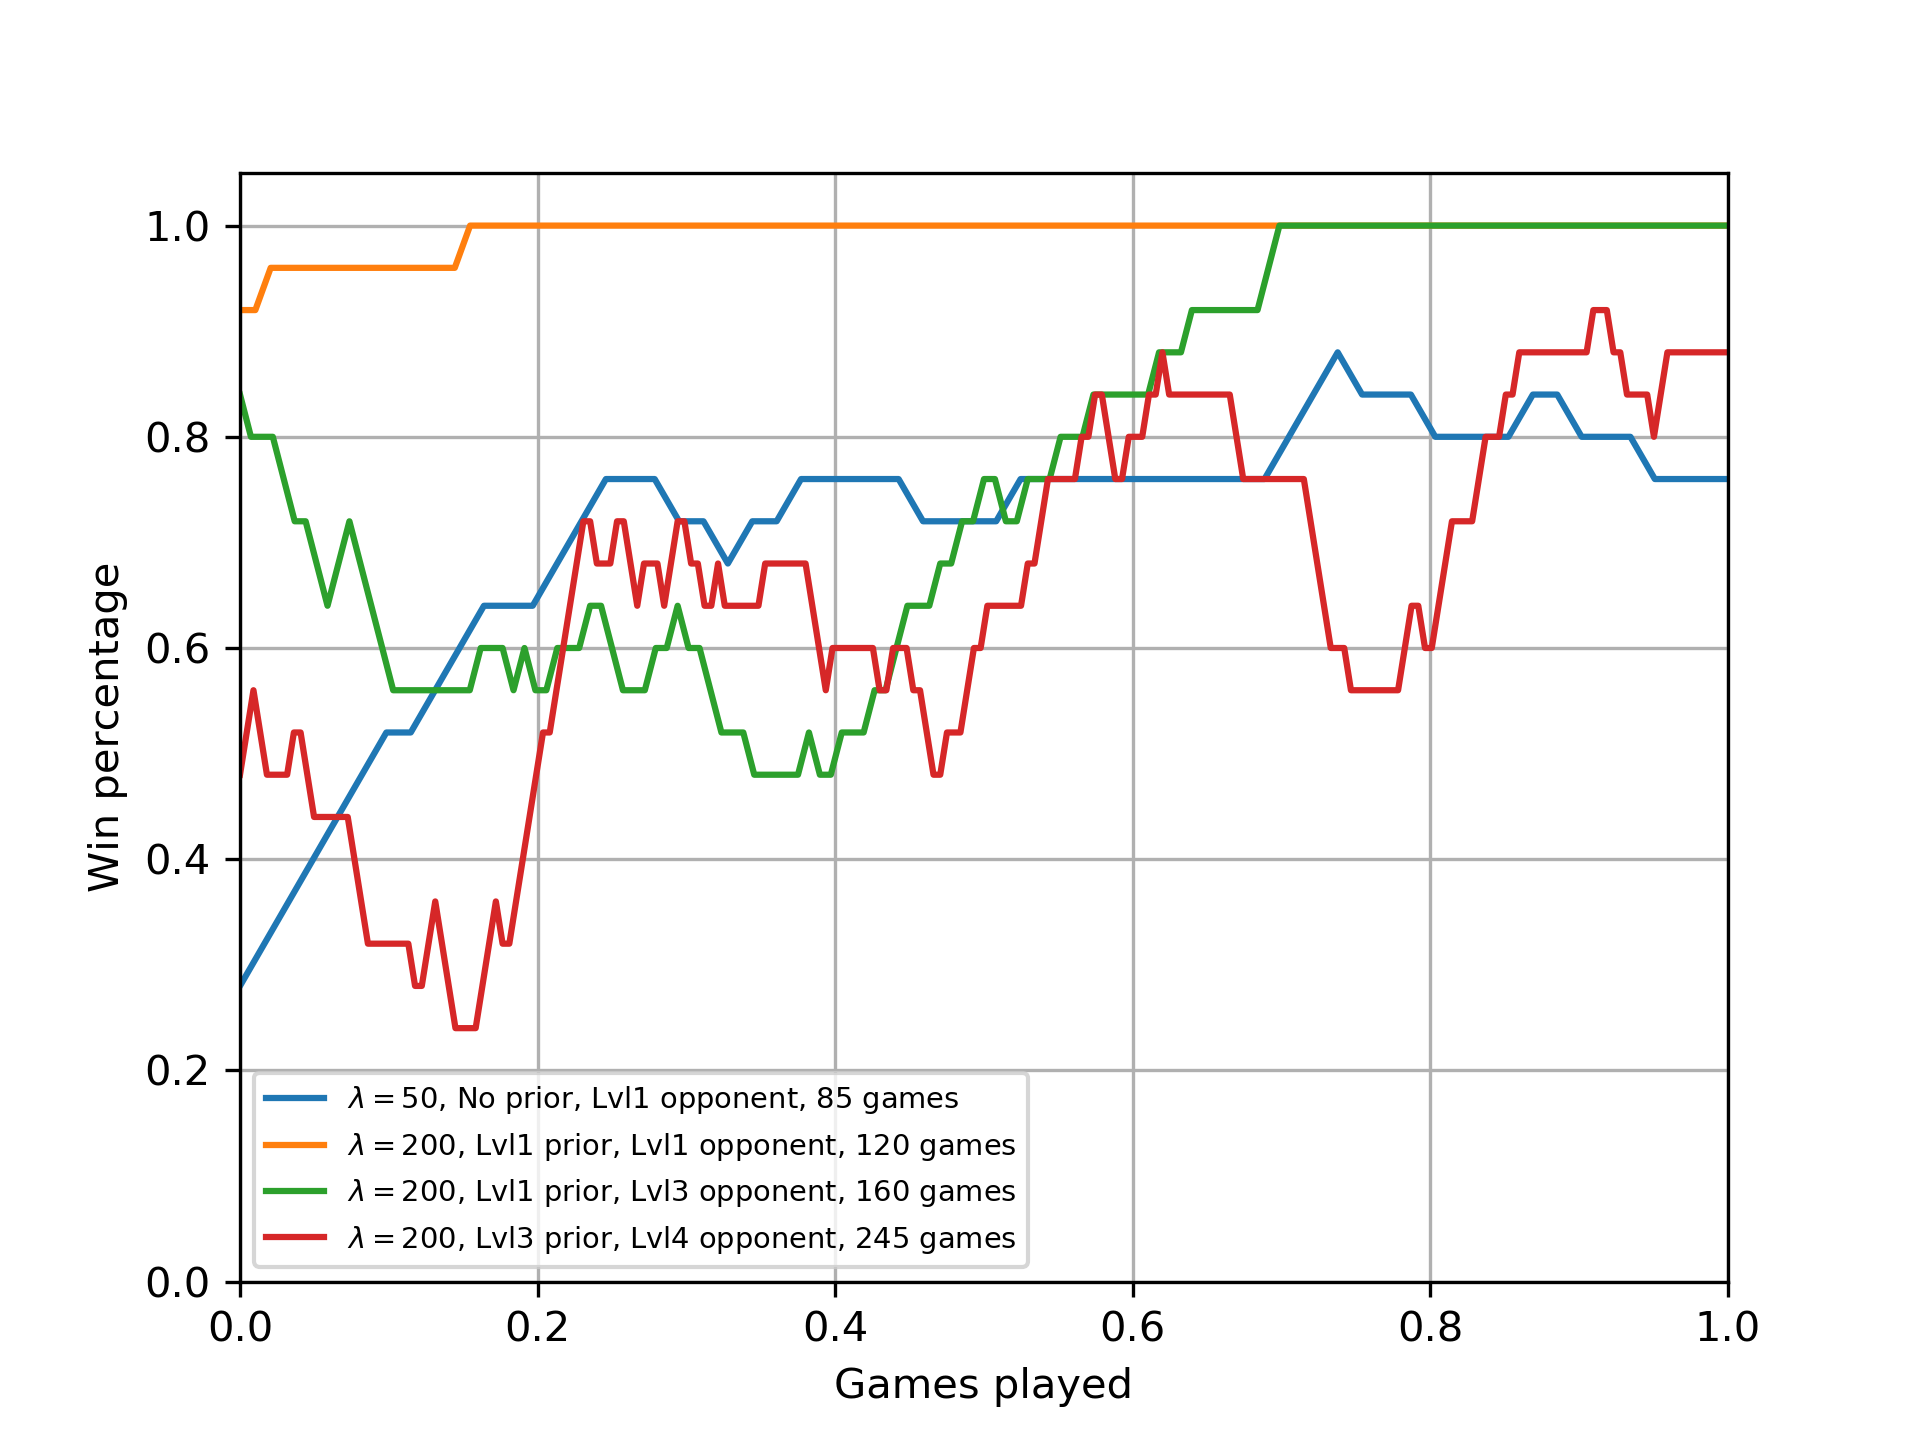
\includegraphics[width=120mm]{winpctg.png}
	\caption{15 game running average of difference in stocks at end of game. \label{winpctg}}
\end{figure}

\begin{figure}[!htb]
\centering
	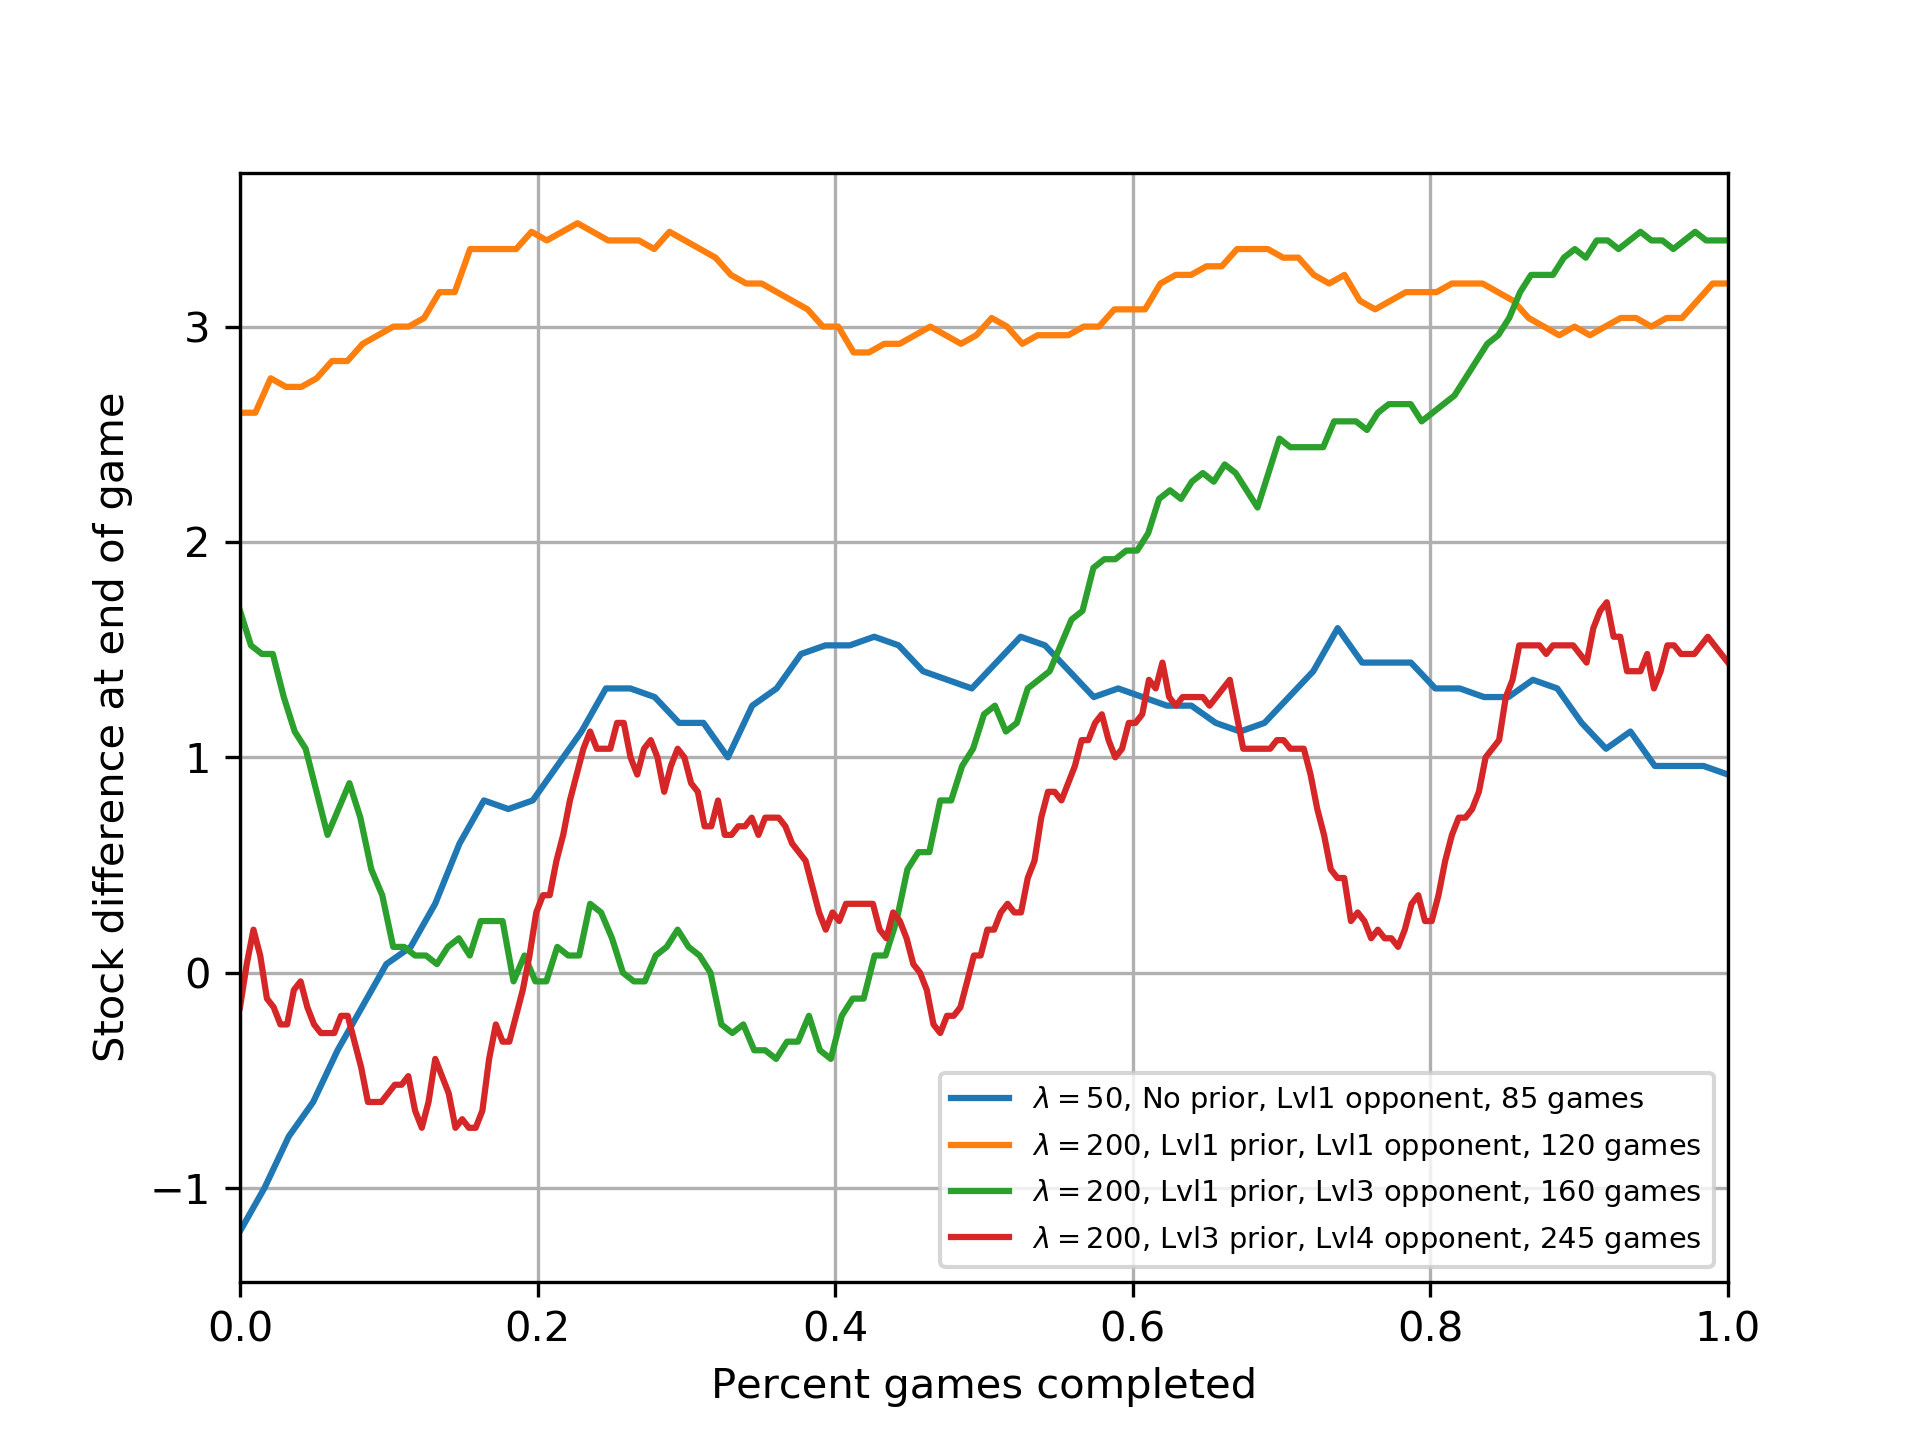
\includegraphics[width=120mm]{stocks.png}
	\caption{15 game running average of difference in stocks at end of game. \label{stocks}}
\end{figure}

\begin{figure}[!htb]
\centering
	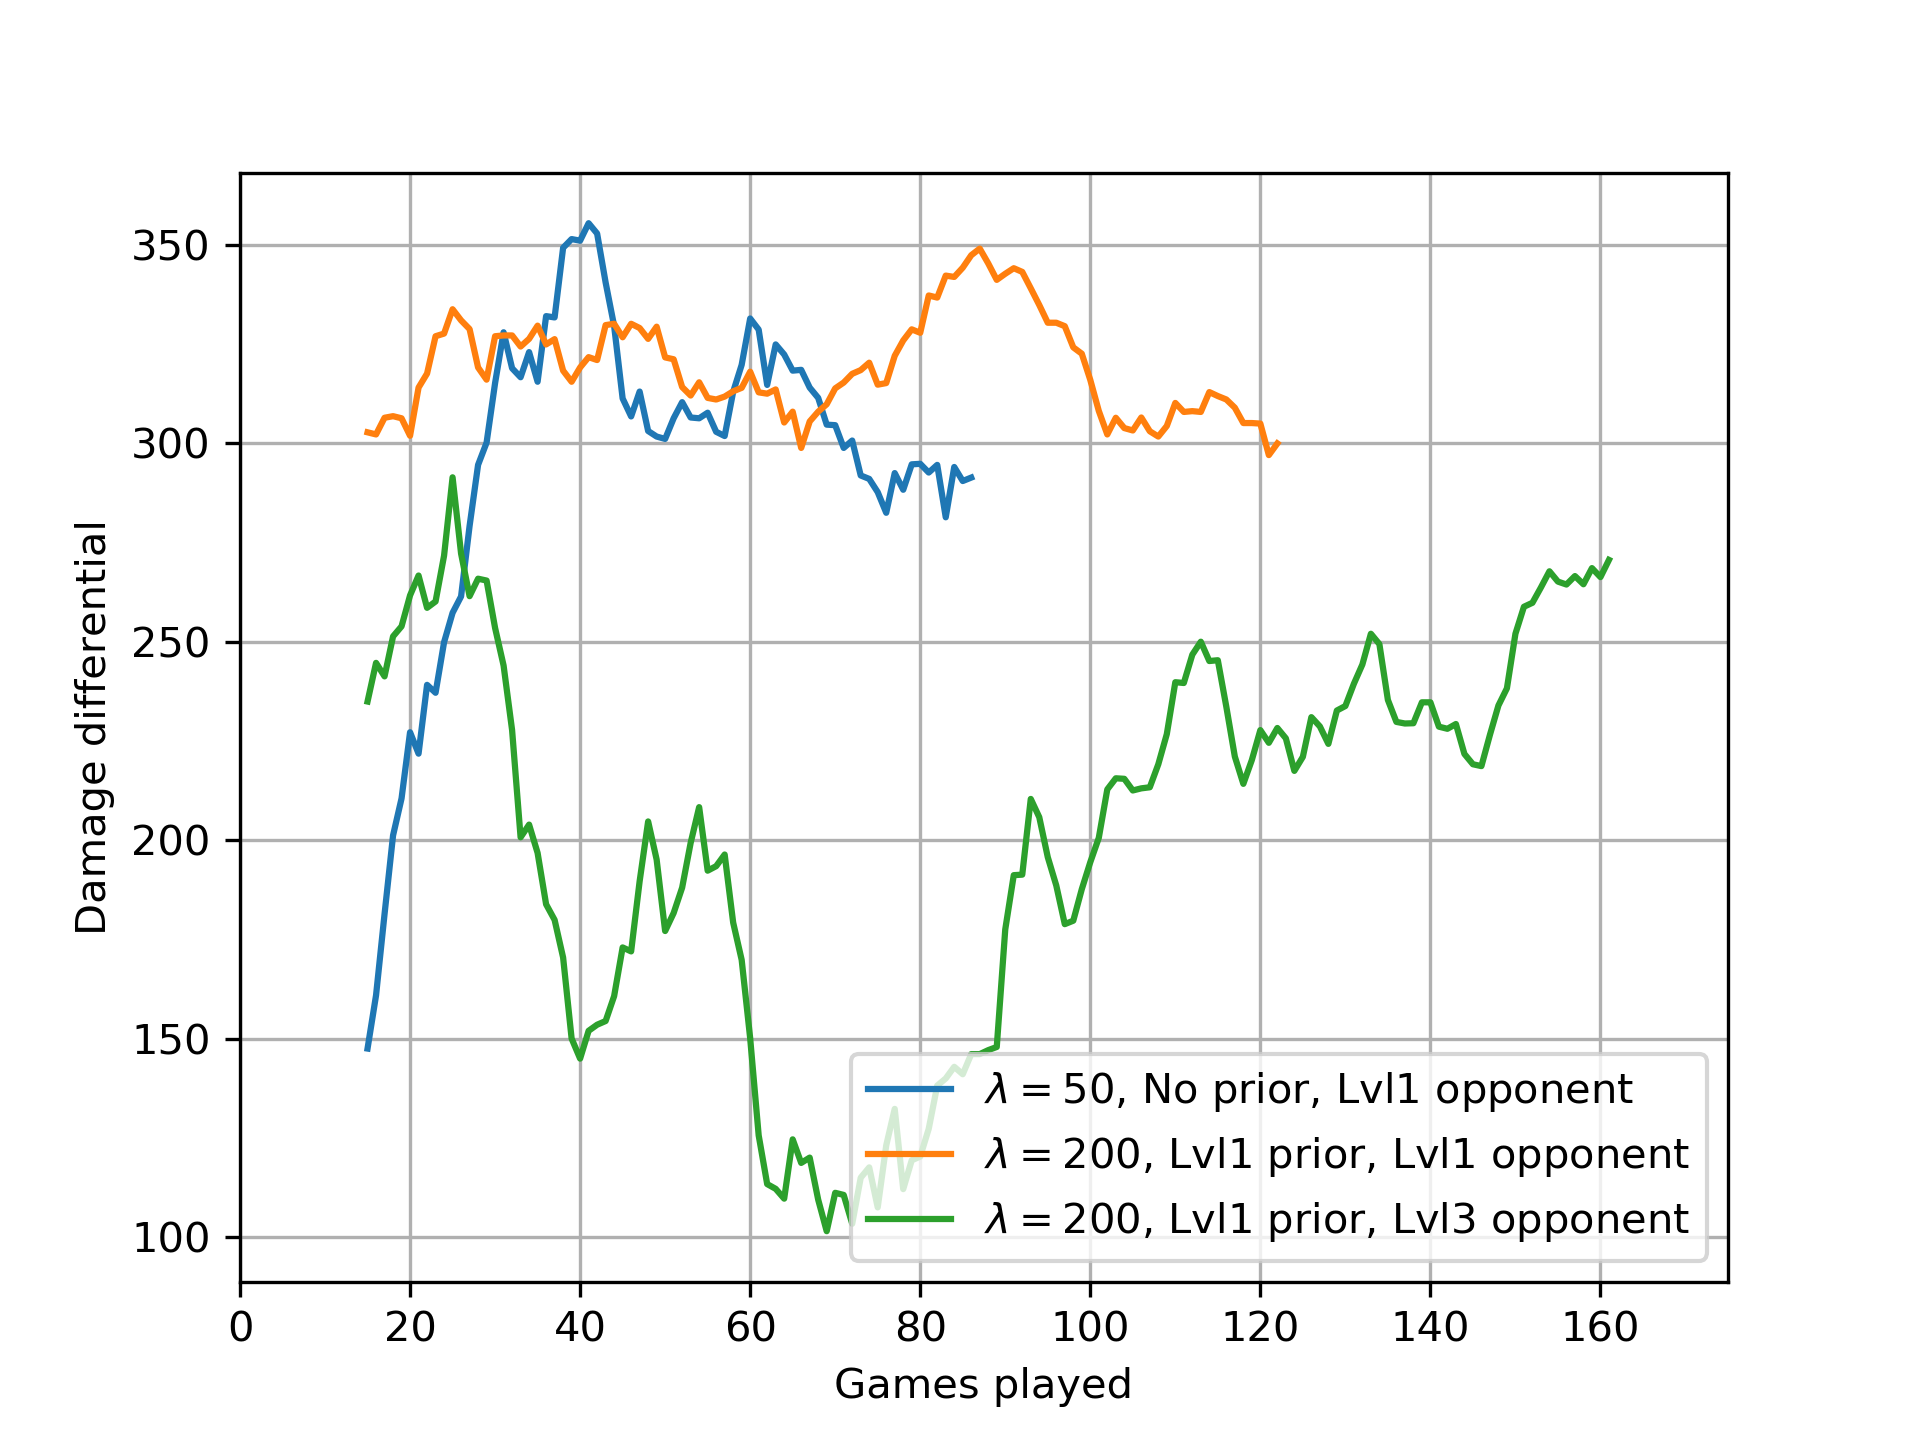
\includegraphics[width=120mm]{damage.png}
	\caption{15 game running average of difference in damage dealt and taken. \label{damage}}
\end{figure}
